\documentclass[a4paper]{scrartcl}
\usepackage[ngerman]{babel}
\usepackage[utf8]{inputenc}
\usepackage[T1]{fontenc}
\usepackage{lmodern}
\usepackage{amssymb}
\usepackage{amsmath}
\usepackage{enumerate}
\usepackage{pgfplots}
\usepackage{scrpage2}\pagestyle{scrheadings}
\usepackage{tikz}
\usepackage{listings}
\usetikzlibrary{patterns}
\input kvmacros 

\newcommand{\titleinfo}{Hausaufgaben zum 7. 12. 2012}
\title{\titleinfo}
\author{Tronje Krabbe 6435002, The-Vinh Jackie Huynh 6388888,\\Arne Struck 6326505}
\date{\today}
\chead{\titleinfo}
\ohead{\today}
\setheadsepline{1pt}
\setcounter{secnumdepth}{0}
\lstset{language=Java}
\newcommand{\qed}{\ \square}
\newcommand{\nand}{\,\overline{\land}\,}

\begin{document}
\maketitle
\notag
\section{1.}
	\subsection{a)}
		\(f(x)=(x_3\vee \overline{x_2})\land (x_2 \vee \overline{x_1})\) \\ \\
		\(
		\begin{array}{c|c|c||c}
				x_1&x_2&x_3&f(x) \\ \hline
				0&0&0&1 \\
				0&0&1&1 \\
				0&1&0&0 \\
				1&0&0&0 \\
				0&1&1&1 \\
				1&1&0&0 \\
				1&0&1&0 \\
				1&1&1&1
		\end{array}
		\) \\ \\
		\(\Rightarrow \textbf{KNF: } 
		(x_1\vee \overline{x_2}\vee x_3)\land
		(\overline{x_1}\vee x_2\vee x_3)\land
		(\overline{x_1}\vee\overline{x_2}\vee x_3)\land
		(\overline{x_1}\vee x_2\vee \overline{x_3})\) \\
		\(\Rightarrow \textbf{DNF: }
		(\overline{x_1}\land\overline{x_2}\land\overline{x_3})\vee
		(\overline{x_1}\land\overline{x_2}\land x_3)\vee
		(\overline{x_1}\land x_2\land x_3)\vee
		(x_1\land x_2\land x_3)\) \\
		\(\Rightarrow\textbf{RMF: }1 \oplus x_2 \oplus x_1 \oplus x_3x_2 \oplus x_2x_1 \) \\ \\
		\newpage
	\subsection{b)}
		\(g(x)=\overline{x_3}\oplus\overline{x_1}\) \\ \\
		\(
		\begin{array}{c|c|c||c}
			x_1&x_2&x_3&f(x) \\ \hline
			0&0&0&0 \\
			0&0&1&1 \\
			0&1&0&0 \\
			1&0&0&1 \\
			0&1&1&1 \\
			1&1&0&1 \\
			1&0&1&0 \\
			1&1&1&0
		\end{array}
		\) \\ \\
		\(\Rightarrow \textbf{KNF: } 
		(x_1\vee x_2\vee x_3)\land
		(x_1\vee \overline{x_2}\vee x_3)\land
		(\overline{x_1}\vee x_2 \vee \overline{x_3})\land
		(\overline{x_1}\vee \overline{x_2}\vee\overline{x_3})\) \\
		\(\Rightarrow \textbf{DNF: } 
		(\overline{x_1}\land\overline{x_2}\land x_3)\vee
		(x_1\land \overline{x_2}\land\overline{x_3})\vee
		(\overline{x_1}\land x_2\land x_3)\vee
		(x_1\land x_2\land x_3)\) \\
		\(\Rightarrow\textbf{RMF: } x_3 \oplus x_1 \) \\

\section{2.}
	\subsection{a)}
		Sei \(\nand\) die Schreibweise für NAND: \\ \\
		\(\begin{array}{c|c|c|c}
			x&\overline{x}&x\land x& x\nand x\\ \hline
			0&1&0&1 \\
			1&0&1&0
		\end{array}\quad\Rightarrow \overline{x}=x\nand x \) \\ \\ \\ \\
		\(\begin{array}{c|c|c|c|c}
			x&y&x\land y & x\nand y &(x\nand y)\nand 
			(x\nand y)\\ \hline
			0&0&0&1&0 \\
			0&1&0&1&0 \\
			1&0&0&1&0 \\
			1&1&1&0&1
		\end{array}\quad\Rightarrow x\land y = (x\nand y)\nand(x\nand y)\overset{*}
		{=}\overline{x\nand y}\) \\ 
		\begin{small}
			* Da die Negation bereits gezeigt wurde, ist dieser Umformungsschritt legitim.
		\end{small} \\ \\ \\
		\(\begin{array}{c|c|c|c|c|c}
			x&y&x\vee y& x\nand x& y\nand y&(x\nand x)\nand(y\nand y)\\ \hline
			0&0&0&1&1&0 \\
			0&1&1&1&0&1 \\
			1&0&1&0&1&1 \\
			1&1&1&0&0&1
		\end{array}\quad\Rightarrow x\vee y = (x\nand x)\nand(y\nand y)\)

	\subsection{b)}
		\begin{align}
			f(x_3,x_2,x_1)&=(\overline{x_3}\land(\overline{x_2}\vee x_1)) \vee 
			(x_1\land(\overline{x_2} \vee x_1)) \\
			&= (\overline{x_2}\vee x_1)\land(\overline{x_3}\vee x_1) \\
			&=x_1\land (\overline{x_2}\vee \overline{x_3}) \\
			&=x_1\land (x_2\nand x_3) \\
			&=\big(x_1\nand(x_2\nand x_3)\big)\nand\big(x_1\nand(x_2\nand x_3)\big)
		\end{align}
		
	
\section{3.}
	\subsection{a)}
		\[\begin{array}{c||c|c|c|c||c|c}
			 &x_3 & x_2 & x_1 & x_0 & \text{A} & \text{B} \\ \hline
			0 & 0 & 0 & 0 & 0 & 1 & 1 \\
			1 & 0 & 0 & 0 & 1 & 0 & 1 \\
			2 & 0 & 0 & 1 & 0 & 1 & 1 \\
			3 & 0 & 0 & 1 & 1 & 1 & 1 \\
			4 & 0 & 1 & 0 & 0 & 0 & 1 \\
			5 & 0 & 1 & 0 & 1 & 1 & 0 \\
			6 & 0 & 1 & 1 & 0 & 1 & 0 \\
			7 & 0 & 1 & 1 & 1 & 1 & 1 \\
			8 & 1 & 0 & 0 & 0 & 1 & 1 \\
			9 & 1 & 0 & 0 & 1 & 1 & 1 \\
		\end{array}\] \\
		
		
		\begin{center}
			\begin{tabular}{ccc}
				A &\quad & B \\
				\begin{tikzpicture}[baseline,x=2em,y=2em]
				
					% Rahmen
					\draw (1,0) node[align=center, minimum size=2em] {\small\text{00}};
					\draw (2,0) node[align=center, minimum size=2em] {\small\text{01}};
					\draw (3,0) node[align=center, minimum size=2em] {\small\text{11}};
					\draw (4,0) node[align=center, minimum size=2em] {\small\text{10}};
					\draw (0,-1) node[align=center, minimum size=2em] {\small\text{00}};
					\draw (0,-2) node[align=center, minimum size=2em] {\small\text{01}};
					\draw (0,-3) node[align=center, minimum size=2em] {\small\text{11}};
					\draw (0,-4) node[align=center, minimum size=2em] {\small\text{10}};
					\draw (-0.5,0.5) -- (0.5,-0.5);
					\draw (-0.25,0.4) node[align=center, minimum size=2em, right] {\small\(x_1x_0\)};
					\draw (-0.7,0.5) node[align=center, minimum size=2em, below] {\small\(x_3x_2\)};
					
					% Inhalt
					% erste Zeile
					\draw (1,-1) node[align=center, draw, minimum size=2em] {1};
					\draw (2,-1) node[align=center, draw, minimum size=2em] {0};
					\draw (3,-1) node[align=center, draw, minimum size=2em] {1};
					\draw (4,-1) node[align=center, draw, minimum size=2em] {1};
					%zeite Zeile
					\draw (1,-2) node[align=center, draw, minimum size=2em] {0};
					\draw (2,-2) node[align=center, draw, minimum size=2em] {1};
					\draw (3,-2) node[align=center, draw, minimum size=2em] {1};
					\draw (4,-2) node[align=center, draw, minimum size=2em] {1};
					%dritte Zeile
					\draw (1,-3) node[align=center, draw, minimum size=2em] {*};
					\draw (2,-3) node[align=center, draw, minimum size=2em] {*};
					\draw (3,-3) node[align=center, draw, minimum size=2em] {*};
					\draw (4,-3) node[align=center, draw, minimum size=2em] {*};
					%vierte Zeile
					\draw (1,-4) node[align=center, draw, minimum size=2em] {1};
					\draw (2,-4) node[align=center, draw, minimum size=2em] {1};
					\draw (3,-4) node[align=center, draw, minimum size=2em] {*};
					\draw (4,-4) node[align=center, draw, minimum size=2em] {*};
				\end{tikzpicture} &\quad &
				
				\begin{tikzpicture}[baseline,x=2em,y=2em]
					% Rahmen
					\draw (1,0) node[align=center, minimum size=2em] (a00) {\small\text{00}};
					\draw (2,0) node[align=center, minimum size=2em] (a01) {\small\text{01}};
					\draw (3,0) node[align=center, minimum size=2em] (a11) {\small\text{11}};
					\draw (4,0) node[align=center, minimum size=2em] (a10) {\small\text{10}};
					\draw (0,-1) node[align=center, minimum size=2em] (b00) {\small\text{00}};
					\draw (0,-2) node[align=center, minimum size=2em] (b01) {\small\text{01}};
					\draw (0,-3) node[align=center, minimum size=2em] (b11) {\small\text{11}};
					\draw (0,-4) node[align=center, minimum size=2em] (b10) {\small\text{10}};
					\draw (-0.5,0.5) -- (0.5,-0.5);
					\draw (-0.25,0.4) node[align=center, minimum size=2em, right] {\small\(x_1x_0\)};
					\draw (-0.7,0.5) node[align=center, minimum size=2em, below] {\small\(x_3x_2\)};
					
					
					% Inhalt
					% erste Zeile
					\draw (1,-1) node[align=center, draw, minimum size=2em] {1};
					\draw (2,-1) node[align=center, draw, minimum size=2em] {1};
					\draw (3,-1) node[align=center, draw, minimum size=2em] {1};
					\draw (4,-1) node[align=center, draw, minimum size=2em] {1};
					%zeite Zeile
					\draw (1,-2) node[align=center, draw, minimum size=2em] {1};
					\draw (2,-2) node[align=center, draw, minimum size=2em] {0};
					\draw (3,-2) node[align=center, draw, minimum size=2em] {1};
					\draw (4,-2) node[align=center, draw, minimum size=2em] {0};
					%dritte Zeile
					\draw (1,-3) node[align=center, draw, minimum size=2em] {*};
					\draw (2,-3) node[align=center, draw, minimum size=2em] {*};
					\draw (3,-3) node[align=center, draw, minimum size=2em] {*};
					\draw (4,-3) node[align=center, draw, minimum size=2em] {*};
					%vierte Zeile
					\draw (1,-4) node[align=center, draw, minimum size=2em] {1};
					\draw (2,-4) node[align=center, draw, minimum size=2em] {1};
					\draw (3,-4) node[align=center, draw, minimum size=2em] {*};
					\draw (4,-4) node[align=center, draw, minimum size=2em] {*};
				\end{tikzpicture}
			\end{tabular}
		\end{center}
	
	\subsection{b)}
		\kvnoindex
		\karnaughmap{4}{A}{{\(x_3\)}{\(x_1\)}{\(x_2\)}{\(x_0\)}}
		{1001 1111 11** ****}
		{
		\begin{tikzpicture}[x=10mm, y=10mm]
			\draw 
			[rounded corners = 1 em, line width = 0.1 em, draw = blue] (3.15,-1.55) rectangle(0,0);
			\draw
			[rounded corners = 1 em, line width = 0.1 em, draw = green](2.3,-0.75) 
			rectangle(0.8,0.8);
			\draw
			[rounded corners = 1 em, line width = 0.1 em, draw = red](3.05,-1.5) rectangle(1.7,1.55);
			\draw 
			[rounded corners = 1 em, line width = 0.1 em, draw = orange] 
			(0,0.9) to (0.7,0.9) to (0.7,1.6);
			\draw
			[rounded corners = 1 em, line width = 0.1 em, draw = orange] 
			(0,-0.85) to (0.7,-0.85) to (0.7,-1.55);
			\draw
			[rounded corners = 1 em, line width = 0.1 em, draw = orange] 
			(3.2,0.9) to (2.45,0.9) to (2.45,1.6);
			\draw			
			[rounded corners = 1 em, line width = 0.1 em, draw = orange] 
			(3.2,-0.8) to (2.45,-0.8) to (2.45,-1.5);
		\end{tikzpicture}
		}
		\karnaughmap{4}{B}{{\(x_3\)}{\(x_1\)}{\(x_2\)}{\(x_0\)}}
		{1110 1110 11** ****}
		{
		\begin{tikzpicture}[x=8.4mm, y=8mm]
			\draw
			[ opacity=1, line width=0.4mm, rounded corners=2mm, draw=red]
            (0.1, 0) to (0.1, 0.9) to (3.9, 0.9) to(3.9, 0)
            (0.1, 4) to (0.1, 3.1) to (3.9, 3.1) to (3.9, 4);
            \draw
            [ opacity=1, line width=0.4mm, rounded corners=2mm, draw=green] 
            (2.2, 0.1) rectangle (2.8, 3.9);
            \draw[ opacity=1, line width=0.4mm, rounded corners=2mm, draw=blue] 
            (0.2, 0.1) rectangle (0.8, 3.9);
		\end{tikzpicture}
		} \\ \\
		\(A(x)= x_3 \vee x_1 \vee (x_2\land x_0)\vee (\overline{x_2}\land\overline{x_0})\) \\
		\(B(x)= \overline{x_2}\vee (\overline{x_1}\land\overline{x_0})\vee (x_1\land x_0)\)

	
\section{4.}	
	\subsection{a)}
		\[
		\begin{array}{c||c|c|c|c||c}
			&x_3 & x_2 & x_1 & x_0 & y \\ \hline 
			0&0 & 0 & 0 & 0 & 0 \\
			1&0 & 0 & 0 & 1 & 0 \\
			2&0 & 0 & 1 & 0 & 0 \\
			3&0 & 0 & 1 & 1 & 0 \\
			4&0 & 1 & 0 & 0 & 0 \\
			5&0 & 1 & 0 & 1 & 1 \\
			6&0 & 1 & 1 & 0 & 0 \\
			7&0 & 1 & 1 & 1 & 1 \\
			8&1 & 0 & 0 & 0 & 0 \\
			9&1 & 0 & 0 & 1 & 0 \\
			10&1 & 0 & 1 & 0 & 0 \\
			11&1 & 0 & 1 & 1 & 0 \\
			12&1 & 1 & 0 & 0 & 1 \\
			13&1 & 1 & 0 & 1 & 1 \\
			14&1 & 1 & 1 & 0 & 1 \\
			15&1 & 1 & 1 & 1 & 1 \\
		\end{array}\] \\
		
	\subsection{b)\& c)}
		\karnaughmap{4}{A}{{\(x_3\)}{\(x_1\)}{\(x_2\)}{\(x_0\)}}
		{0001 0001 0011 0011}
		{
		\begin{tikzpicture}[x=8.4mm, y=8mm]
			\draw 
			[rounded corners = 1 em, line width = 0 em, draw = blue] (0,0) rectangle(0,0);
            \draw
            [ opacity=1, line width=0.4mm, rounded corners=2mm, draw=green] 
            (0.1, 1.2) rectangle (3.7, 1.8);
            \draw[ opacity=1, line width=0.4mm, rounded corners=2mm, draw=blue] 
            (1.1, 1.1) rectangle (2.75, 2.9);
		\end{tikzpicture}
		} \(\quad y= (x_3\land x_2)\vee(x_0\land x_2)\)
	
	\subsection{d)}
		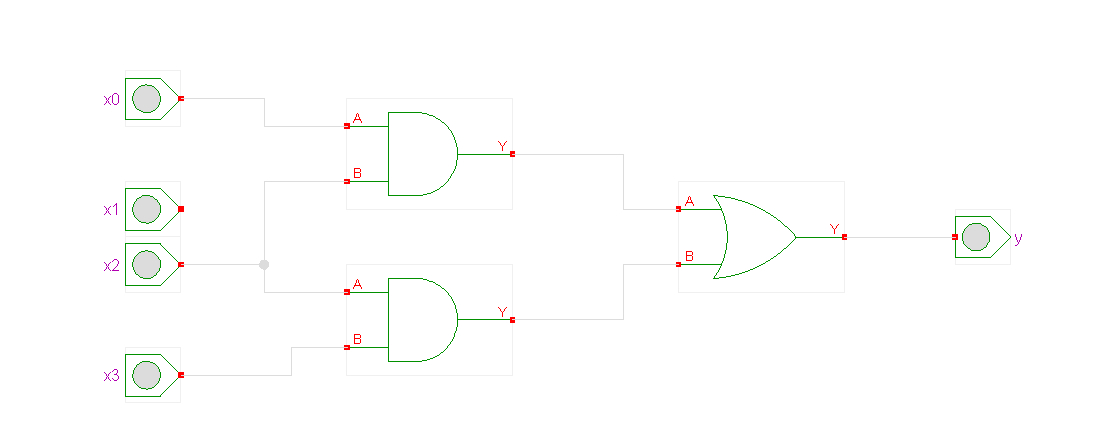
\includegraphics[scale=0.55]{splan.png}
	

\end{document}